% Options for packages loaded elsewhere
\PassOptionsToPackage{unicode}{hyperref}
\PassOptionsToPackage{hyphens}{url}
%
\documentclass[
  ignorenonframetext,
]{beamer}
\usepackage{pgfpages}
\setbeamertemplate{caption}[numbered]
\setbeamertemplate{caption label separator}{: }
\setbeamercolor{caption name}{fg=normal text.fg}
\beamertemplatenavigationsymbolsempty
% Prevent slide breaks in the middle of a paragraph
\widowpenalties 1 10000
\raggedbottom
\setbeamertemplate{part page}{
  \centering
  \begin{beamercolorbox}[sep=16pt,center]{part title}
    \usebeamerfont{part title}\insertpart\par
  \end{beamercolorbox}
}
\setbeamertemplate{section page}{
  \centering
  \begin{beamercolorbox}[sep=12pt,center]{part title}
    \usebeamerfont{section title}\insertsection\par
  \end{beamercolorbox}
}
\setbeamertemplate{subsection page}{
  \centering
  \begin{beamercolorbox}[sep=8pt,center]{part title}
    \usebeamerfont{subsection title}\insertsubsection\par
  \end{beamercolorbox}
}
\AtBeginPart{
  \frame{\partpage}
}
\AtBeginSection{
  \ifbibliography
  \else
    \frame{\sectionpage}
  \fi
}
\AtBeginSubsection{
  \frame{\subsectionpage}
}

\usepackage{amsmath,amssymb}
\usepackage{iftex}
\ifPDFTeX
  \usepackage[T1]{fontenc}
  \usepackage[utf8]{inputenc}
  \usepackage{textcomp} % provide euro and other symbols
\else % if luatex or xetex
  \usepackage{unicode-math}
  \defaultfontfeatures{Scale=MatchLowercase}
  \defaultfontfeatures[\rmfamily]{Ligatures=TeX,Scale=1}
\fi
\usepackage{lmodern}
\ifPDFTeX\else  
    % xetex/luatex font selection
\fi
% Use upquote if available, for straight quotes in verbatim environments
\IfFileExists{upquote.sty}{\usepackage{upquote}}{}
\IfFileExists{microtype.sty}{% use microtype if available
  \usepackage[]{microtype}
  \UseMicrotypeSet[protrusion]{basicmath} % disable protrusion for tt fonts
}{}
\makeatletter
\@ifundefined{KOMAClassName}{% if non-KOMA class
  \IfFileExists{parskip.sty}{%
    \usepackage{parskip}
  }{% else
    \setlength{\parindent}{0pt}
    \setlength{\parskip}{6pt plus 2pt minus 1pt}}
}{% if KOMA class
  \KOMAoptions{parskip=half}}
\makeatother
\usepackage{xcolor}
\newif\ifbibliography
\setlength{\emergencystretch}{3em} % prevent overfull lines
\setcounter{secnumdepth}{-\maxdimen} % remove section numbering

\usepackage{color}
\usepackage{fancyvrb}
\newcommand{\VerbBar}{|}
\newcommand{\VERB}{\Verb[commandchars=\\\{\}]}
\DefineVerbatimEnvironment{Highlighting}{Verbatim}{commandchars=\\\{\}}
% Add ',fontsize=\small' for more characters per line
\usepackage{framed}
\definecolor{shadecolor}{RGB}{241,243,245}
\newenvironment{Shaded}{\begin{snugshade}}{\end{snugshade}}
\newcommand{\AlertTok}[1]{\textcolor[rgb]{0.68,0.00,0.00}{#1}}
\newcommand{\AnnotationTok}[1]{\textcolor[rgb]{0.37,0.37,0.37}{#1}}
\newcommand{\AttributeTok}[1]{\textcolor[rgb]{0.40,0.45,0.13}{#1}}
\newcommand{\BaseNTok}[1]{\textcolor[rgb]{0.68,0.00,0.00}{#1}}
\newcommand{\BuiltInTok}[1]{\textcolor[rgb]{0.00,0.23,0.31}{#1}}
\newcommand{\CharTok}[1]{\textcolor[rgb]{0.13,0.47,0.30}{#1}}
\newcommand{\CommentTok}[1]{\textcolor[rgb]{0.37,0.37,0.37}{#1}}
\newcommand{\CommentVarTok}[1]{\textcolor[rgb]{0.37,0.37,0.37}{\textit{#1}}}
\newcommand{\ConstantTok}[1]{\textcolor[rgb]{0.56,0.35,0.01}{#1}}
\newcommand{\ControlFlowTok}[1]{\textcolor[rgb]{0.00,0.23,0.31}{#1}}
\newcommand{\DataTypeTok}[1]{\textcolor[rgb]{0.68,0.00,0.00}{#1}}
\newcommand{\DecValTok}[1]{\textcolor[rgb]{0.68,0.00,0.00}{#1}}
\newcommand{\DocumentationTok}[1]{\textcolor[rgb]{0.37,0.37,0.37}{\textit{#1}}}
\newcommand{\ErrorTok}[1]{\textcolor[rgb]{0.68,0.00,0.00}{#1}}
\newcommand{\ExtensionTok}[1]{\textcolor[rgb]{0.00,0.23,0.31}{#1}}
\newcommand{\FloatTok}[1]{\textcolor[rgb]{0.68,0.00,0.00}{#1}}
\newcommand{\FunctionTok}[1]{\textcolor[rgb]{0.28,0.35,0.67}{#1}}
\newcommand{\ImportTok}[1]{\textcolor[rgb]{0.00,0.46,0.62}{#1}}
\newcommand{\InformationTok}[1]{\textcolor[rgb]{0.37,0.37,0.37}{#1}}
\newcommand{\KeywordTok}[1]{\textcolor[rgb]{0.00,0.23,0.31}{#1}}
\newcommand{\NormalTok}[1]{\textcolor[rgb]{0.00,0.23,0.31}{#1}}
\newcommand{\OperatorTok}[1]{\textcolor[rgb]{0.37,0.37,0.37}{#1}}
\newcommand{\OtherTok}[1]{\textcolor[rgb]{0.00,0.23,0.31}{#1}}
\newcommand{\PreprocessorTok}[1]{\textcolor[rgb]{0.68,0.00,0.00}{#1}}
\newcommand{\RegionMarkerTok}[1]{\textcolor[rgb]{0.00,0.23,0.31}{#1}}
\newcommand{\SpecialCharTok}[1]{\textcolor[rgb]{0.37,0.37,0.37}{#1}}
\newcommand{\SpecialStringTok}[1]{\textcolor[rgb]{0.13,0.47,0.30}{#1}}
\newcommand{\StringTok}[1]{\textcolor[rgb]{0.13,0.47,0.30}{#1}}
\newcommand{\VariableTok}[1]{\textcolor[rgb]{0.07,0.07,0.07}{#1}}
\newcommand{\VerbatimStringTok}[1]{\textcolor[rgb]{0.13,0.47,0.30}{#1}}
\newcommand{\WarningTok}[1]{\textcolor[rgb]{0.37,0.37,0.37}{\textit{#1}}}

\providecommand{\tightlist}{%
  \setlength{\itemsep}{0pt}\setlength{\parskip}{0pt}}\usepackage{longtable,booktabs,array}
\usepackage{calc} % for calculating minipage widths
\usepackage{caption}
% Make caption package work with longtable
\makeatletter
\def\fnum@table{\tablename~\thetable}
\makeatother
\usepackage{graphicx}
\makeatletter
\def\maxwidth{\ifdim\Gin@nat@width>\linewidth\linewidth\else\Gin@nat@width\fi}
\def\maxheight{\ifdim\Gin@nat@height>\textheight\textheight\else\Gin@nat@height\fi}
\makeatother
% Scale images if necessary, so that they will not overflow the page
% margins by default, and it is still possible to overwrite the defaults
% using explicit options in \includegraphics[width, height, ...]{}
\setkeys{Gin}{width=\maxwidth,height=\maxheight,keepaspectratio}
% Set default figure placement to htbp
\makeatletter
\def\fps@figure{htbp}
\makeatother

\makeatletter
\@ifpackageloaded{caption}{}{\usepackage{caption}}
\AtBeginDocument{%
\ifdefined\contentsname
  \renewcommand*\contentsname{Table of contents}
\else
  \newcommand\contentsname{Table of contents}
\fi
\ifdefined\listfigurename
  \renewcommand*\listfigurename{List of Figures}
\else
  \newcommand\listfigurename{List of Figures}
\fi
\ifdefined\listtablename
  \renewcommand*\listtablename{List of Tables}
\else
  \newcommand\listtablename{List of Tables}
\fi
\ifdefined\figurename
  \renewcommand*\figurename{Figure}
\else
  \newcommand\figurename{Figure}
\fi
\ifdefined\tablename
  \renewcommand*\tablename{Table}
\else
  \newcommand\tablename{Table}
\fi
}
\@ifpackageloaded{float}{}{\usepackage{float}}
\floatstyle{ruled}
\@ifundefined{c@chapter}{\newfloat{codelisting}{h}{lop}}{\newfloat{codelisting}{h}{lop}[chapter]}
\floatname{codelisting}{Listing}
\newcommand*\listoflistings{\listof{codelisting}{List of Listings}}
\makeatother
\makeatletter
\makeatother
\makeatletter
\@ifpackageloaded{caption}{}{\usepackage{caption}}
\@ifpackageloaded{subcaption}{}{\usepackage{subcaption}}
\makeatother
\ifLuaTeX
  \usepackage{selnolig}  % disable illegal ligatures
\fi
\usepackage{bookmark}

\IfFileExists{xurl.sty}{\usepackage{xurl}}{} % add URL line breaks if available
\urlstyle{same} % disable monospaced font for URLs
\hypersetup{
  pdftitle={Пакет targets},
  pdfauthor={Егор Глушков DTwin},
  hidelinks,
  pdfcreator={LaTeX via pandoc}}

\title{Пакет targets}
\author{Егор ГлушковDTwin}
\date{2024-09-09}

\begin{document}
\frame{\titlepage}

\begin{frame}{Проблема №1}
\phantomsection\label{ux43fux440ux43eux431ux43bux435ux43cux430-1}
\begin{itemize}
\item
  Новый проект с огромной кодовой базой: десятки файлов, тысячи строк
  кода
\item
  Поменять один параметр, ``достать'' часть данных
\item
  Как \emph{это} запускать? Как понять зависимости между
  файлами/функциями?
\end{itemize}
\end{frame}

\begin{frame}{Проблема №2}
\phantomsection\label{ux43fux440ux43eux431ux43bux435ux43cux430-2}
\begin{itemize}
\item
  Разобрались со связями: есть несколько моделей, которые зависят от
  разных наборов данных
\item
  Поменялся один из наборов данных или изменились параметры модели --
  пересобирать весь проект \textbf{\emph{заново}}?
\end{itemize}

\begin{itemize}[<+->]
\item
  Спустя часы выполнения возникла ошибка в маленьком малозначимом
  кусочке кода?

  \begin{figure}[H]

  {\centering 
\includegraphics[width=3.125in,height=\textheight]{Sources/pepe.jpg}

  }

  \caption{Ошибка? Спустя несколько часов выполнения?}

  \end{figure}%
\end{itemize}
\end{frame}

\begin{frame}{Проблема №3}
\phantomsection\label{ux43fux440ux43eux431ux43bux435ux43cux430-3}
\begin{itemize}
\item
  Нашли, какую модель надо перезапустить, а какую не надо
\item
  Как сохранить результаты моделей так, чтобы они не менялись, когда не
  меняется вход?
\item
  Как посмотреть вход или выход тех или иных функций?
\end{itemize}
\end{frame}

\begin{frame}{Решение проблем}
\phantomsection\label{ux440ux435ux448ux435ux43dux438ux435-ux43fux440ux43eux431ux43bux435ux43c}
\begin{block}{\textbf{T A R G E T S}}
\phantomsection\label{t-a-r-g-e-t-s}
\begin{figure}[H]

{\centering 
\includegraphics{Sources/logo.png}

}

\caption{Targets -- и ваша жизнь не будет прежней}

\end{figure}%
\end{block}
\end{frame}

\begin{frame}{Материалы}
\phantomsection\label{ux43cux430ux442ux435ux440ux438ux430ux43bux44b}
\begin{itemize}
\item
  \href{https://books.ropensci.org/targets/}{The \{targets\} R package
  user manual} -- материалы отсюда
\item
  \href{https://github.com/ropensci/targets}{Targets package on Github}
\item
  Get started with \{targets\} in 4 minutes
  \url{https://vimeo.com/700982360}
\end{itemize}
\end{frame}

\begin{frame}[fragile]{Особенности}
\phantomsection\label{ux43eux441ux43eux431ux435ux43dux43dux43eux441ux442ux438}
\begin{itemize}
\item
  Принцип схож с \texttt{makefile}
\item
  В основе лежит функционально-ориентированный стиль (как и во всем R)
\item
  Весь код представлен как последовательность узлов (\emph{aka
  таргетов}), сходных с функциями, у которых есть вход и выход. Таргеты
  зависят друг от друга
\item
  Ключевой файл -- \texttt{\_targets.R}. В нем содержится список всех
  таргетов. Всегда должен находиться в корне папки
\end{itemize}
\end{frame}

\begin{frame}{Типичная структура проекта}
\phantomsection\label{ux442ux438ux43fux438ux447ux43dux430ux44f-ux441ux442ux440ux443ux43aux442ux443ux440ux430-ux43fux440ux43eux435ux43aux442ux430}
├── \_targets.R

├── 01.Data/data.csv

├── 02.R/

│~~ ├── 01.functions.R

│~~ ├── 02.\ldots{}

├── 03.Targets/

│~~ ├── 01.tar1.R

│~~ ├── 02.\ldots{}
\end{frame}

\begin{frame}[fragile]{С чего начинать? {[}1/2{]}}
\phantomsection\label{ux441-ux447ux435ux433ux43e-ux43dux430ux447ux438ux43dux430ux442ux44c-12}
\begin{enumerate}
\item
  Написать код как некоторую последовательность функций в R (pipeline),
  сохранить в папку с кодом \texttt{/02.R/}
\item
  Вызвать \texttt{use\_targets()} для создания ключевого файла
  \texttt{\_targets.R}
\item
  Заполнить \texttt{\_targets.R} нужными таргетами, не забыв загрузить
  библиотеки, глобальные переменные и функции
\end{enumerate}
\end{frame}

\begin{frame}[fragile]{С чего начинать? {[}2/2{]}}
\phantomsection\label{ux441-ux447ux435ux433ux43e-ux43dux430ux447ux438ux43dux430ux442ux44c-22}
\begin{enumerate}
\setcounter{enumi}{3}
\tightlist
\item
  При первом запуске для создания метаданных использовать tar\_make(). В
  дальнейшем для просмотра графа связей
  \texttt{tar\_visnetwork()}\footnote<.->{Или лучше
    \texttt{tar\_visnetwork(targets\_only\ =\ TRUE)}}
\item
  Результат выполнения в папке \texttt{/\_targets/}. Просмотр
  посчитанных таргетов: \texttt{tar\_read(01.My\_first\_target)}
\end{enumerate}
\end{frame}

\begin{frame}[fragile]{Файл \_targets.R {[}1/2{]}}
\phantomsection\label{ux444ux430ux439ux43b-_targets.r-12}
Классический \texttt{\_targets.R} содержит:

\begin{itemize}
\item
  загружаемые пакеты
\item
  \texttt{tar\_option\_set()}
\item
  \texttt{source("01.R/functions.R")}
\item
  список таргетов: \texttt{list(tar\_target(…),\ tar\_target(…),\ …)}
\end{itemize}
\end{frame}

\begin{frame}[fragile]{Файл \_targets.R {[}2/2{]}}
\phantomsection\label{ux444ux430ux439ux43b-_targets.r-22}
\begin{Shaded}
\begin{Highlighting}[]
\FunctionTok{source}\NormalTok{(}\StringTok{"01.Targets/01.Libraries.R"}\NormalTok{)}
\FunctionTok{source}\NormalTok{(}\StringTok{"01.Targets/02.Functions.R"}\NormalTok{)}
\FunctionTok{source}\NormalTok{(}\StringTok{"01.Targets/03.List\_of\_targets.R"}\NormalTok{)}


\FunctionTok{tar\_option\_set}\NormalTok{(}\AttributeTok{format =} \StringTok{"qs"}\NormalTok{)}
\FunctionTok{tar\_config\_set}\NormalTok{(}\AttributeTok{script =} \StringTok{"\_targets.R"}\NormalTok{, }\AttributeTok{store =} \StringTok{"\_targets"}\NormalTok{)}


\FunctionTok{list}\NormalTok{(}
\NormalTok{  data\_targets,}
\NormalTok{  ANOVA\_targets,}
\NormalTok{  PCA\_targets}
\NormalTok{)}
\end{Highlighting}
\end{Shaded}
\end{frame}

\begin{frame}[fragile]{Файл 03.List\_of\_targets.R {[}1/2{]}}
\phantomsection\label{ux444ux430ux439ux43b-03.list_of_targets.r-12}
\begin{Shaded}
\begin{Highlighting}[]
\NormalTok{PCA\_targets }\OtherTok{\textless{}{-}} \FunctionTok{list}\NormalTok{(}
  \FunctionTok{tar\_target}\NormalTok{(DT.}\DecValTok{03}\NormalTok{.}\FloatTok{1.}\NormalTok{PCA\_model,}
             \FunctionTok{calculate\_PCA\_model}\NormalTok{(DT.}\DecValTok{01}\NormalTok{.}\FloatTok{1.}\NormalTok{Get\_data, }\AttributeTok{scale =} \ConstantTok{TRUE}\NormalTok{)),}

  \FunctionTok{tar\_target}\NormalTok{(DT.}\DecValTok{03}\NormalTok{.}\FloatTok{2.}\NormalTok{PCA\_summary,}
             \FunctionTok{pca\_summary}\NormalTok{(DT.}\DecValTok{03}\NormalTok{.}\FloatTok{1.}\NormalTok{PCA\_model)),}

  \FunctionTok{tar\_target}\NormalTok{(DT.}\DecValTok{03}\NormalTok{.}\FloatTok{3.}\NormalTok{PCA\_loadings,}
             \FunctionTok{pca\_loadings}\NormalTok{(DT.}\DecValTok{03}\NormalTok{.}\FloatTok{1.}\NormalTok{PCA\_model)),}

  \FunctionTok{tar\_target}\NormalTok{(DT.}\DecValTok{03}\NormalTok{.}\FloatTok{4.}\NormalTok{PCA\_plot,}
             \FunctionTok{plot\_to\_pdf}\NormalTok{(DT.}\DecValTok{03}\NormalTok{.}\FloatTok{1.}\NormalTok{PCA\_model, }\StringTok{"PCA\_components"}\NormalTok{)),}

  \FunctionTok{tar\_target}\NormalTok{(DT.}\DecValTok{03}\NormalTok{.}\FloatTok{5.}\NormalTok{PCA\_less\_dim,}
             \FunctionTok{pca\_plot\_lesser\_dim}\NormalTok{(DT.}\DecValTok{01}\NormalTok{.}\FloatTok{1.}\NormalTok{Get\_data, }\StringTok{"Species"}\NormalTok{))}
\NormalTok{)}
\end{Highlighting}
\end{Shaded}
\end{frame}

\begin{frame}[fragile]{Файл 03.List\_of\_targets.R {[}2/2{]}}
\phantomsection\label{ux444ux430ux439ux43b-03.list_of_targets.r-22}
\begin{Shaded}
\begin{Highlighting}[]
\NormalTok{data\_targets }\OtherTok{\textless{}{-}} \FunctionTok{list}\NormalTok{(}
  \FunctionTok{tar\_target}\NormalTok{(DT.}\DecValTok{01}\NormalTok{.}\FloatTok{1.}\NormalTok{Get\_data,}
             \FunctionTok{get\_data}\NormalTok{(}\AttributeTok{data =}\NormalTok{ iris, }\AttributeTok{slice\_n =} \ConstantTok{NULL}\NormalTok{)),}

  \FunctionTok{tar\_target}\NormalTok{(DT.}\DecValTok{01}\NormalTok{.}\FloatTok{2.}\NormalTok{Plot\_pairs,}
             \FunctionTok{plot\_pairs}\NormalTok{(DT.}\DecValTok{01}\NormalTok{.}\FloatTok{1.}\NormalTok{Get\_data))}
\NormalTok{)}


\NormalTok{ANOVA\_targets }\OtherTok{\textless{}{-}} \FunctionTok{list}\NormalTok{(}
  \FunctionTok{tar\_target}\NormalTok{(DT.}\DecValTok{02}\NormalTok{.}\FloatTok{1.}\NormalTok{ANOVA\_model,}
             \FunctionTok{calculate\_anova\_model}\NormalTok{(DT.}\DecValTok{01}\NormalTok{.}\FloatTok{1.}\NormalTok{Get\_data))}
\NormalTok{)}
\end{Highlighting}
\end{Shaded}
\end{frame}

\begin{frame}[fragile]{Файл 02.Functions.R {[}1/2{]}}
\phantomsection\label{ux444ux430ux439ux43b-02.functions.r-12}
\begin{Shaded}
\begin{Highlighting}[]
\CommentTok{\# 1. Getting data           \#\#\#\#}
\NormalTok{get\_data }\OtherTok{\textless{}{-}} \ControlFlowTok{function}\NormalTok{(}\AttributeTok{data =}\NormalTok{ iris, }\AttributeTok{slice\_n =} \ConstantTok{NULL}\NormalTok{) \{}
  \ControlFlowTok{if}\NormalTok{ (}\SpecialCharTok{!}\FunctionTok{is.null}\NormalTok{(slice\_n)) \{}
    \FunctionTok{return}\NormalTok{(data[slice\_n,])}
\NormalTok{  \} }\ControlFlowTok{else}\NormalTok{ \{}
    \FunctionTok{return}\NormalTok{(data)}
\NormalTok{  \}}
\NormalTok{\}}


\CommentTok{\# 2. Models                 \#\#\#\#}
\CommentTok{\# 2.1 ANOVA model           \#\#\#\#}
\NormalTok{calculate\_anova\_model }\OtherTok{\textless{}{-}} \ControlFlowTok{function}\NormalTok{(}\AttributeTok{data\_ =}\NormalTok{ iris) \{}
\NormalTok{  r }\OtherTok{\textless{}{-}} \FunctionTok{aov}\NormalTok{(}\FunctionTok{lm}\NormalTok{(data\_[, }\DecValTok{1}\NormalTok{] }\SpecialCharTok{\textasciitilde{}}\NormalTok{ ., }\AttributeTok{data =}\NormalTok{ data\_[}\SpecialCharTok{{-}}\DecValTok{1}\NormalTok{]))}
  \FunctionTok{return}\NormalTok{(}\FunctionTok{summary}\NormalTok{(r))}
\NormalTok{\}}


\CommentTok{\# 2.2 PCA model             \#\#\#\#}
\NormalTok{calculate\_PCA\_model }\OtherTok{\textless{}{-}} \ControlFlowTok{function}\NormalTok{(data\_, }\AttributeTok{scale =} \ConstantTok{TRUE}\NormalTok{) \{}
\NormalTok{  pca\_data }\OtherTok{\textless{}{-}}\NormalTok{ data\_ }\SpecialCharTok{\%\textgreater{}\%}
    \FunctionTok{as.data.table}\NormalTok{() }\SpecialCharTok{\%\textgreater{}\%}
    \FunctionTok{copy}\NormalTok{()}
\NormalTok{  pca\_data }\OtherTok{\textless{}{-}} \ControlFlowTok{if}\NormalTok{ (scale) \{}
\NormalTok{    pca\_data[, }\FunctionTok{scale}\NormalTok{(.SD), .SDcols }\OtherTok{=}\NormalTok{ is.numeric]}
\NormalTok{  \} }\ControlFlowTok{else}\NormalTok{ \{}
\NormalTok{    pca\_data[, .SD, .SDcols }\OtherTok{=}\NormalTok{ is.numeric]}
\NormalTok{  \}}
  \FunctionTok{return}\NormalTok{(pca\_data }\SpecialCharTok{\%\textgreater{}\%} \FunctionTok{princomp}\NormalTok{())}
\NormalTok{\}}
\end{Highlighting}
\end{Shaded}
\end{frame}

\begin{frame}[fragile]{Файл 02.Functions.R {[}1/2{]}}
\phantomsection\label{ux444ux430ux439ux43b-02.functions.r-12-1}
\begin{Shaded}
\begin{Highlighting}[]
\NormalTok{pca\_summary }\OtherTok{\textless{}{-}}\NormalTok{ \textbackslash{}(pca\_res) pca\_res }\SpecialCharTok{\%\textgreater{}\%} \FunctionTok{summary}\NormalTok{()}
\NormalTok{pca\_loadings }\OtherTok{\textless{}{-}}\NormalTok{ \textbackslash{}(pca\_res) pca\_res }\SpecialCharTok{\%\textgreater{}\%} \FunctionTok{loadings}\NormalTok{()}

\NormalTok{plot\_to\_pdf }\OtherTok{\textless{}{-}} \ControlFlowTok{function}\NormalTok{(pca\_res, }\AttributeTok{file\_name =} \StringTok{"my\_plot"}\NormalTok{) \{}
  \FunctionTok{pdf}\NormalTok{(}\FunctionTok{paste0}\NormalTok{(}\StringTok{"02.Outputs/"}\NormalTok{, file\_name, }\StringTok{".pdf"}\NormalTok{))}
\NormalTok{  pca\_res }\SpecialCharTok{\%\textgreater{}\%} \FunctionTok{plot}\NormalTok{()}
  \FunctionTok{dev.off}\NormalTok{()}
  \FunctionTok{return}\NormalTok{(}\FunctionTok{invisible}\NormalTok{(}\ConstantTok{NULL}\NormalTok{))}
\NormalTok{\}}


\CommentTok{\# 2.3 Another PCA model      \#\#\#\#}
\NormalTok{pca\_plot\_lesser\_dim }\OtherTok{\textless{}{-}} \ControlFlowTok{function}\NormalTok{(data\_, factor\_var, }\AttributeTok{file\_name =} \StringTok{"PCA\_less\_dim"}\NormalTok{) \{}
\NormalTok{  pca\_res }\OtherTok{\textless{}{-}}\NormalTok{ data\_ }\SpecialCharTok{\%\textgreater{}\%}
    \FunctionTok{as.data.table}\NormalTok{() }\SpecialCharTok{\%\textgreater{}\%}
    \FunctionTok{copy}\NormalTok{() }\SpecialCharTok{\%\textgreater{}\%}
\NormalTok{    .[, }\FunctionTok{scale}\NormalTok{(.SD), .SDcols }\OtherTok{=}\NormalTok{ is.numeric] }\SpecialCharTok{\%\textgreater{}\%}
\NormalTok{    ade4}\SpecialCharTok{::}\FunctionTok{dudi.pca}\NormalTok{(}\AttributeTok{scannf=}\ConstantTok{FALSE}\NormalTok{)}

  \FunctionTok{pdf}\NormalTok{(}\FunctionTok{paste0}\NormalTok{(}\StringTok{"02.Outputs/"}\NormalTok{, file\_name, }\StringTok{".pdf"}\NormalTok{))}
\NormalTok{  ade4}\SpecialCharTok{::}\FunctionTok{s.class}\NormalTok{(pca\_res}\SpecialCharTok{$}\NormalTok{li, data\_[, factor\_var])}
  \FunctionTok{dev.off}\NormalTok{()}

  \FunctionTok{return}\NormalTok{(}\FunctionTok{invisible}\NormalTok{(}\ConstantTok{NULL}\NormalTok{))}
\NormalTok{\}}


\CommentTok{\# 2.4 Another plot functions        \#\#\#\#}
\NormalTok{plot\_pairs }\OtherTok{\textless{}{-}}\NormalTok{ \textbackslash{}(data\_, }\AttributeTok{file\_name =} \StringTok{"pairs\_plot"}\NormalTok{) \{}
  \FunctionTok{pdf}\NormalTok{(}\FunctionTok{paste0}\NormalTok{(}\StringTok{"02.Outputs/"}\NormalTok{, file\_name, }\StringTok{".pdf"}\NormalTok{))}
\NormalTok{  data\_ }\SpecialCharTok{\%\textgreater{}\%} \FunctionTok{pairs}\NormalTok{()}
  \FunctionTok{dev.off}\NormalTok{()}
  \FunctionTok{return}\NormalTok{(}\FunctionTok{invisible}\NormalTok{(}\ConstantTok{NULL}\NormalTok{))}
\NormalTok{\}}
\end{Highlighting}
\end{Shaded}
\end{frame}

\begin{frame}[fragile]{Команды: \texttt{tar\_manifest}}
\phantomsection\label{ux43aux43eux43cux430ux43dux434ux44b-tar_manifest}
\begin{itemize}
\item
  \texttt{tar\_manifest()}

\begin{Shaded}
\begin{Highlighting}[]
\FunctionTok{tar\_manifest}\NormalTok{(}\AttributeTok{fields =} \FunctionTok{all\_of}\NormalTok{(}\StringTok{"command"}\NormalTok{))}
\end{Highlighting}
\end{Shaded}

\begin{verbatim}
# A tibble: 8 × 2
  name                 command                                              
  <chr>                <chr>                                                
1 DT.01.1.Get_data     "get_data(data = iris, slice_n = NULL)"              
2 DT.03.5.PCA_less_dim "pca_plot_lesser_dim(DT.01.1.Get_data, \"Species\")" 
3 DT.03.1.PCA_model    "calculate_PCA_model(DT.01.1.Get_data, scale = TRUE)"
4 DT.01.2.Plot_pairs   "plot_pairs(DT.01.1.Get_data)"                       
5 DT.02.1.ANOVA_model  "calculate_anova_model(DT.01.1.Get_data)"            
6 DT.03.2.PCA_summary  "pca_summary(DT.03.1.PCA_model)"                     
7 DT.03.3.PCA_loadings "pca_loadings(DT.03.1.PCA_model)"                    
8 DT.03.4.PCA_plot     "plot_to_pdf(DT.03.1.PCA_model, \"PCA_components\")" 
\end{verbatim}
\end{itemize}
\end{frame}

\begin{frame}[fragile]{Команды: \texttt{tar\_visnetwork}}
\phantomsection\label{ux43aux43eux43cux430ux43dux434ux44b-tar_visnetwork}
\begin{itemize}
\item
  \texttt{tar\_visnetwork(targets\_only\ =\ TRUE)}

  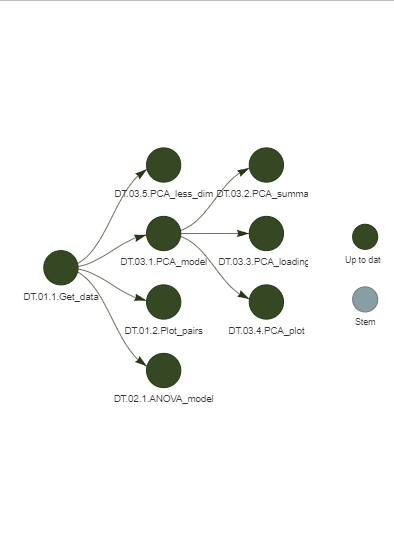
\includegraphics{Sources/up_target.png}
\end{itemize}
\end{frame}

\begin{frame}[fragile]{Команды: \texttt{tar\_visnetwork}}
\phantomsection\label{ux43aux43eux43cux430ux43dux434ux44b-tar_visnetwork-1}
\begin{itemize}
\item
  \texttt{tar\_visnetwork(targets\_only\ =\ TRUE)} после изменения
  параметров одного из узлов

  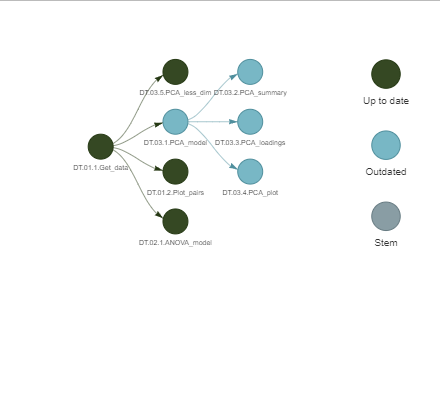
\includegraphics[width=5.20833in,height=\textheight]{Sources/outdated_target.png}
\end{itemize}
\end{frame}

\begin{frame}[fragile]{Команды: \texttt{tar\_make}, \texttt{tar\_read}}
\phantomsection\label{ux43aux43eux43cux430ux43dux434ux44b-tar_make-tar_read}
\begin{itemize}
\item
  \texttt{tar\_make()}

\begin{verbatim}
✔ skipped target DT.01.1.Get_data
✔ skipped target DT.03.5.PCA_less_dim 
✔ skipped target DT.03.1.PCA_model 
✔ skipped target DT.01.2.Plot_pairs 
✔ skipped target DT.02.1.ANOVA_model
✔ skipped target DT.03.2.PCA_summary
✔ skipped target DT.03.3.PCA_loadings
✔ skipped target DT.03.4.PCA_plot
✔ skipped pipeline [0.188 seconds]
\end{verbatim}
\item
  \texttt{tar\_read(DT.01.1.Get\_data)}

\begin{verbatim}
    Sepal.Length Sepal.Width Petal.Length Petal.Width    Species 
    1            5.1         3.5          1.4         0.2     setosa
    2            4.9         3.0          1.4         0.2     setosa
    3            4.7         3.2          1.3         0.2     setosa
    4            4.6         3.1          1.5         0.2     setosa
\end{verbatim}
\end{itemize}
\end{frame}

\begin{frame}[fragile]{Полезные команды: \texttt{tar\_cue}}
\phantomsection\label{ux43fux43eux43bux435ux437ux43dux44bux435-ux43aux43eux43cux430ux43dux434ux44b-tar_cue}
\begin{itemize}
\item
  \texttt{tar\_cue()}

\begin{Shaded}
\begin{Highlighting}[]
\FunctionTok{tar\_target}\NormalTok{(DT.}\FloatTok{01.}\NormalTok{Download\_target, }\FunctionTok{download\_data}\NormalTok{(), }\AttributeTok{cue =} \FunctionTok{tar\_cue}\NormalTok{(}\AttributeTok{mode =} \StringTok{"always"}\NormalTok{))}
\end{Highlighting}
\end{Shaded}

\begin{Shaded}
\begin{Highlighting}[]
\FunctionTok{tar\_cue}\NormalTok{(}
  \AttributeTok{mode =} \FunctionTok{c}\NormalTok{(}\StringTok{"thorough"}\NormalTok{, }\StringTok{"always"}\NormalTok{, }\StringTok{"never"}\NormalTok{),}
  \AttributeTok{command =} \ConstantTok{TRUE}\NormalTok{,}
  \AttributeTok{depend =} \ConstantTok{TRUE}\NormalTok{,}
  \AttributeTok{format =} \ConstantTok{TRUE}\NormalTok{,}
  \AttributeTok{repository =} \ConstantTok{TRUE}\NormalTok{,}
  \AttributeTok{iteration =} \ConstantTok{TRUE}\NormalTok{,}
  \AttributeTok{file =} \ConstantTok{TRUE}\NormalTok{,}
  \AttributeTok{seed =} \ConstantTok{TRUE}
\NormalTok{)}
\end{Highlighting}
\end{Shaded}
\item
  Cue mode. If~\texttt{"thorough"}, all the cues apply unless
  individually suppressed. If~\texttt{"always"}, then the target always
  runs. If~\texttt{"never"}, then the target does not run unless the
  metadata does not exist or the last run errored.
\end{itemize}
\end{frame}

\begin{frame}[fragile]{Отслеживание изменений {[}1/2{]}}
\phantomsection\label{ux43eux442ux441ux43bux435ux436ux438ux432ux430ux43dux438ux435-ux438ux437ux43cux435ux43dux435ux43dux438ux439-12}
\begin{itemize}
\item
  Для отслеживания изменений \texttt{targets} считает \emph{hash}: так,
  изменение тела функции, аргументов, зависимостей влечет и изменение
  хэша
\item
  Объект должен быть совместим с форматом хранения, выбранным с помощью
  аргумента \texttt{format}~функций \texttt{tar\_target()} или
  \texttt{tar\_option\_set()}
\end{itemize}
\end{frame}

\begin{frame}[fragile]{Отслеживание изменений {[}2/2{]}}
\phantomsection\label{ux43eux442ux441ux43bux435ux436ux438ux432ux430ux43dux438ux435-ux438ux437ux43cux435ux43dux435ux43dux438ux439-22}
\begin{itemize}
\item
  Не все изменения отслеживаются -\textgreater{}
  \href{https://cran.r-project.org/web/packages/future/vignettes/future-4-non-exportable-objects.html}{Non-Exportable
  Objects}:

  \begin{itemize}
  \item
    base::connection, DBIconnection
  \item
    cpp, Rcpp, rJava, reticulate, keras, polars, xgboost
  \item
    parallel, arrow tables, sparklyr
  \item
    XML
  \end{itemize}
\item
  Для таких объектов или существуют обходные пути, или стоит просто
  принять: изменение этих объектов не всегда влечет автоматическое
  обнаружение этих изменений пакетом \texttt{targets}
\end{itemize}
\end{frame}

\begin{frame}{Каким должен быть tar\_target? {[}1/2{]}}
\phantomsection\label{ux43aux430ux43aux438ux43c-ux434ux43eux43bux436ux435ux43d-ux431ux44bux442ux44c-tar_target-12}
Хороший target обычно:

\begin{enumerate}
\item
  Достаточно крупный, чтобы при пропуске (\emph{skipped}) значительно
  сократить время выполнения
\item
  Достаточно мал, чтобы некоторые таргеты можно было пропустить, даже
  если другие необходимо перевыполнить
\end{enumerate}
\end{frame}

\begin{frame}[fragile]{Каким должен быть tar\_target? {[}2/2{]}}
\phantomsection\label{ux43aux430ux43aux438ux43c-ux434ux43eux43bux436ux435ux43d-ux431ux44bux442ux44c-tar_target-22}
\begin{enumerate}
\setcounter{enumi}{2}
\tightlist
\item
  Не вызывает побочных эффектов, таких как изменения глобальной среды
  (не касается, например, target с
  \texttt{tar\_target(format\ =\ "file")})
\item
  Возвращает единственное значение, которое:

  \begin{enumerate}
  [i.]
  \item
    Легко понять и проанализировать
  \item
    Значимое для проекта
  \item
    Легко сохранить как файл, например, с помощью \texttt{qsave()}.
    Следует избегать неэкспортируемых объектов (см. предыдущий слайд)
  \end{enumerate}
\end{enumerate}
\end{frame}

\begin{frame}[fragile]{Динамическое и статическое ветвление}
\phantomsection\label{ux434ux438ux43dux430ux43cux438ux447ux435ux441ux43aux43eux435-ux438-ux441ux442ux430ux442ux438ux447ux435ux441ux43aux43eux435-ux432ux435ux442ux432ux43bux435ux43dux438ux435}
\begin{longtable}[]{@{}
  >{\raggedright\arraybackslash}p{(\columnwidth - 2\tabcolsep) * \real{0.4444}}
  >{\raggedright\arraybackslash}p{(\columnwidth - 2\tabcolsep) * \real{0.5556}}@{}}
\toprule\noalign{}
\begin{minipage}[b]{\linewidth}\raggedright
Dynamic
\end{minipage} & \begin{minipage}[b]{\linewidth}\raggedright
Static
\end{minipage} \\
\midrule\noalign{}
\endhead
Pipeline creates new targets at runtime & All targets defined in
advance \\
Cryptic target names & Friendly target names \\
Scales to hundreds of branches & Does not scale as easily for
\texttt{tar\_visnetwork()} etc \\
No metaprogramming required & Familiarity with metaprogramming is
helpful \\
\bottomrule\noalign{}
\end{longtable}
\end{frame}

\begin{frame}[fragile]{Пакет tarchetypes {[}1/3{]}}
\phantomsection\label{ux43fux430ux43aux435ux442-tarchetypes-13}
\begin{itemize}
\item
  \href{https://docs.ropensci.org/tarchetypes/}{Ссылка} на пакет
\item
  Позволяет создавать таргеты сложной структуры и с особой
  функциональностью:

  \begin{itemize}
  \item
    Dynamic branching:

    \begin{itemize}
    \item
      over subsets of data frames: \texttt{tar\_group\_by()},
      \texttt{tar\_group\_select()}, etc\ldots{}
    \item
      over files: \texttt{tar\_files()}
    \item
      dynamic batched replication: \texttt{tar\_rep()}
    \item
      dynamic batched replication within static branches for data
      frames: \texttt{tar\_map\_rep()}
    \end{itemize}
  \end{itemize}
\end{itemize}
\end{frame}

\begin{frame}[fragile]{Пакет tarchetypes {[}2/3{]}}
\phantomsection\label{ux43fux430ux43aux435ux442-tarchetypes-23}
\begin{itemize}
\item
  \begin{itemize}
  \item
    Static branching:

    \begin{itemize}
    \item
      \texttt{tar\_combine()}
    \item
      \texttt{tar\_map()}
    \end{itemize}
  \item
    Позволяет создавать таргеты сложной структуры и с особой
    функциональностью:

    \begin{itemize}
    \item
      создание \emph{rmd/quatro}-отчетов:
      \texttt{tar\_render(report,\ "report.Rmd")}
    \item
      Amazon Web Services (AWS):

      \begin{itemize}
      \tightlist
      \item
        \texttt{tar\_aws\_file()}, \texttt{tar\_aws\_parquet()},
        etc\ldots{}
      \end{itemize}
    \end{itemize}
  \end{itemize}
\end{itemize}
\end{frame}

\begin{frame}[fragile]{Пакет tarchetypes {[}3/3{]}}
\phantomsection\label{ux43fux430ux43aux435ux442-tarchetypes-33}
\begin{itemize}
\item
  \begin{itemize}
  \item
    \texttt{tar\_url()}, \texttt{tar\_file()},
    \texttt{tar\_file\_fast()}
  \item
    Особые модели и форматы: \texttt{tar\_keras()},
    \texttt{tar\_torch()}, \texttt{tar\_format\_feather()}
  \item
    Сохранение в объектные файлы напрямую: \texttt{tar\_parquet()},
    \texttt{tar\_fst()}, \texttt{tar\_fst\_dt()},
    \texttt{tar\_fst\_tbl()}, \texttt{tar\_rds()}, \texttt{tar\_qs()}
  \end{itemize}
\end{itemize}
\end{frame}

\begin{frame}[fragile]{Очистка локального хранилища вычисленных
таргетов}
\phantomsection\label{ux43eux447ux438ux441ux442ux43aux430-ux43bux43eux43aux430ux43bux44cux43dux43eux433ux43e-ux445ux440ux430ux43dux438ux43bux438ux449ux430-ux432ux44bux447ux438ux441ux43bux435ux43dux43dux44bux445-ux442ux430ux440ux433ux435ux442ux43eux432}
\begin{itemize}
\item
  \texttt{tar\_destroy()} удаляет \texttt{\_targets/}
\item
  \texttt{tar\_prune()} удаляет данные и метадату, не относящуюся к
  текущему пайплайну в \texttt{\_targets.R}
\item
  \texttt{tar\_delete()} удаляет конкретный файл из
  \texttt{\_targets/objects/} без изменения метадаты
\item
  \texttt{tar\_invalidate()} удаляет метадату из таргетса, но оставляет
  связанные с таргетом данные в \texttt{\_targets/objects/}
\item
  \texttt{tar\_meta\_delete()} удаляет \texttt{\_targets/meta/}
\end{itemize}
\end{frame}

\begin{frame}[fragile]{Некоторые заметки}
\phantomsection\label{ux43dux435ux43aux43eux442ux43eux440ux44bux435-ux437ux430ux43cux435ux442ux43aux438}
\begin{itemize}
\item
  Один targets может быть использован некоторыми проектами (как targets
  по городам)
\item
  Для повторяемости исследования при наличии случайности следует
  фиксировать \emph{seed}: \texttt{tar\_option\_set(seed\ =\ 42)}
\item
  Есть возможность писать список \texttt{tar\_target()} как ячейки в
  \texttt{rmd} 😱 -\textgreater{}
  \href{https://books.ropensci.org/targets/literate-programming.html}{Literate
  programming}
\item
  \texttt{Targets} можно вычислять распределенно на нескольких
  вычислителях -\textgreater{}
  \href{https://books.ropensci.org/targets/crew.html}{Distributed
  computing}
\end{itemize}
\end{frame}

\begin{frame}[fragile]{Ускорение работы \texttt{targets}}
\phantomsection\label{ux443ux441ux43aux43eux440ux435ux43dux438ux435-ux440ux430ux431ux43eux442ux44b-targets}
\begin{itemize}
\item
  Для ускорения работы:

  \begin{itemize}
  \item
    \texttt{tar\_option\_set(format\ =\ "qs")}
  \item
    \texttt{tar\_option\_set(memory\ =\ "transient",\ garbage\_collection\ =\ TRUE)}
  \end{itemize}
\end{itemize}
\end{frame}

\begin{frame}[fragile]{Предостережение}
\phantomsection\label{ux43fux440ux435ux434ux43eux441ux442ux435ux440ux435ux436ux435ux43dux438ux435}
Не стоит запускать \texttt{tar\_make()} в крупных проектах (например,
проекты 123, 207, 211), где уже записан \texttt{targets}. Это может
стоить очень долго и дорого
\end{frame}

\begin{frame}[fragile]{Домашнее задание}
\phantomsection\label{ux434ux43eux43cux430ux448ux43dux435ux435-ux437ux430ux434ux430ux43dux438ux435}
\begin{itemize}
\item
  Сделать \texttt{targets} из задания про \texttt{kmeans}. Минимум
  четыре осмысленных таргета
\item
  Результат:

  \begin{itemize}
  \item
    оформленный код с \texttt{targets}
  \item
    сохраненный граф всех узлов (\emph{html})
  \item
    указание \emph{(можно комментарием в коде)}, где лежит результат
    применения модели и как эти данные можно прочитать
  \end{itemize}
\end{itemize}
\end{frame}



\end{document}
